\section{Evaluation}\label{sec:evaluation}

The evaluation of our preemption point placement algorithm will embody
two methods: 1) characterization and measurement of preemption costs
using real-time application code, and 2) a schedulability comparison
of synthetic task set for various preemption models. 

\subsection {Preemption Cost
  Characterization}\label{sec:preemption_cost_measurement} 
To characterize the behavior and estimate the benefit of the approach
proposed in this paper, a case study of representative tasks was
performed. The tasks were selected from Malardalen University of
Sweden's WCET benchmark suite \cite{mrtc:01}. Each task was built using Gaisler's
Bare-C Cross Compiler \cite{gaisler:01} for the GRSIM
LEON3 \cite{gaisler:02} simulated target. 

Within a task, variance in the number of shared UCBs between program
points is related to the execution flow of the task through each of
the points. For instance, one path to ${P_j}$ may include only ${P_h}$,
while another path to ${P_j}$ may contain ${P_h}$ followed by
${P_i}$. The set of UCBs shared between ${P_h}$ and ${P_j}$ may differ
based on the path between them. If the paths differ one of them may
result in a greater number of shared UCBs between the points. To
accurately upper-bound the shared UCBs between points requires
complete control flow information.

Tasks were first analyzed using AbsInt's a\textsuperscript{3} WCET
\cite{absint:01} to determine the set of basic blocks. Next, the basic
blocks ${\{B_1, B_2, ..., B_n\}}$ were serialized based upon an
understanding of the control flow of the task. Program points ${\{P_1,
  P_2, ..., P_n\}}$ were assigned by setting ${P_i}$ to the address of
the final instruction of each basic block ${B_i}$ for ${i}$ from ${0}$
to ${n}$.

Each program point ${P_j}$ served as a breakpoint when running the
task on the simulator. As the task was executed, at each breakpoint
${P_j}$, the instruction and data cache states were saved as ${I_j}$
and ${D_j}$. Given the limitations of the simulator and
a\textsuperscript{3} it was not possible record the actual control
flow. Thus, calculating an accurate over-estimate of the UCBs shared
between program points was not possible. A selection of cache
snapshots were chosen to representation the actual behavior.

The representative cache contents were selected as the final visit of
each program point. A program point ${P_i}$ may be visited multiple
times during a tasks execution. The UCBs shared between ${P_i}$ and a
later point ${P_j}$ could change with each visit of ${P_i}$. During
the final visit of ${P_i}$ the instruction and data cache contents
were snapshotted, and recorded as ${I_i}$ and ${D_i}$. From these
representative snapshots, a representative over-estimate of shared
UCBs were made. 

Shared UCBs were calculated by intersecting the cache state from ${P_i}$
to ${P_j}$, except ${P_j}$. A cache line that remains unchanged after
the execution of ${\langle}$ ${P_i}$, ${P_{i+1}}$, ..., ${P_{j-1}}$
${\rangle}$ will be
present in the cache before execution of the basic block that ${P_j}$
represents. It is only from these unchanged cache lines that the shared UCBs
between ${P_i}$ and ${P_j}$ can be selected. The complete set of
unchanged cache lines serves as a safe upper-bound on the shared UCBs
between the two points. The equation below formalizes this idea, using
${H}$ as either the set of instruction cache or data cache snapshots.

\begin{center}
  \begin{equation*}
    UCB(P_i, P_j) = \bigcap_{k=i}^{j-1} H_k
  \end{equation*}
\end{center}

\subsubsection{Availability}

This method may be verified and reproduced using the same tools and
data. Gaisler's compiler and simulator are freely available. AbsInt's
a\textsuperscript{3} tool is available for educational and evaluation
purposes. The programs written and data used in this paper can be
found on GitHub at the following url:

\begin{center}
https://github.com/ctessler/superblocks/tree/master/study
\end{center}


\subsubsection{Results}

The results are presented as a comparison between the our proposed
method and the Bertonga approach. For a program point ${P_j}$ the 
Bertogna \cite{bertogna:11} approach defines the UCBs (and therefor the CRPD) as:

\begin{equation*}
  \max\{ UCB(P_i, P_j) \vert i < j \}
\end{equation*}

To determine the maximum benefit of the new approach, the best case
scenario is considered. When the preemption point is selected with the
fewest number of UCBs based upon previous preemption.  For ${P_j}$ the
determination is made by:

\begin{equation*}
  \min\{ UCB(P_i, P_j) \vert i < j \}
\end{equation*}


In the following graphs, each point in the graph represents two points
in the program. The first point of the program ${P_i}$ is fixed by the
x-axis. Each point in the graph is labelled with a number, a later
program point ${P_j}$ which has been selected by the the Bertogna
approach, or by the proposed method. Bertogna's approach follows the
dashed blue line, the proposed approach the solid black line.

Bertogna's approach is represented by the dashed blue line. The proposed
approach by the solid black line. Both approaches will select two
program points, represented by a single position in the
graph. Bertogna's approach would select the lowest value of the dashed
blue line. The proposed approach would select the lowest value of the
solid black line. Comparing the number of shared UCBs allows a
comparison to be made.

\begin{center}
  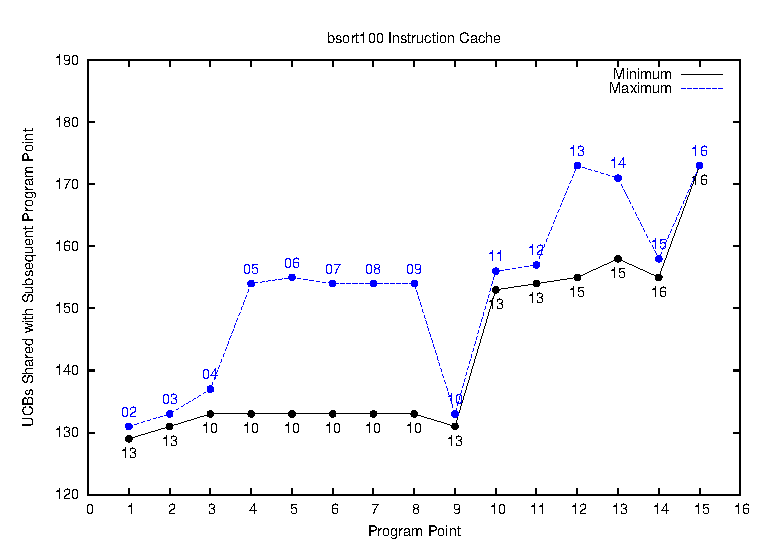
\includegraphics[width=\linewidth]{eps/bsort-icache.eps}
\end{center}

\begin{center}
  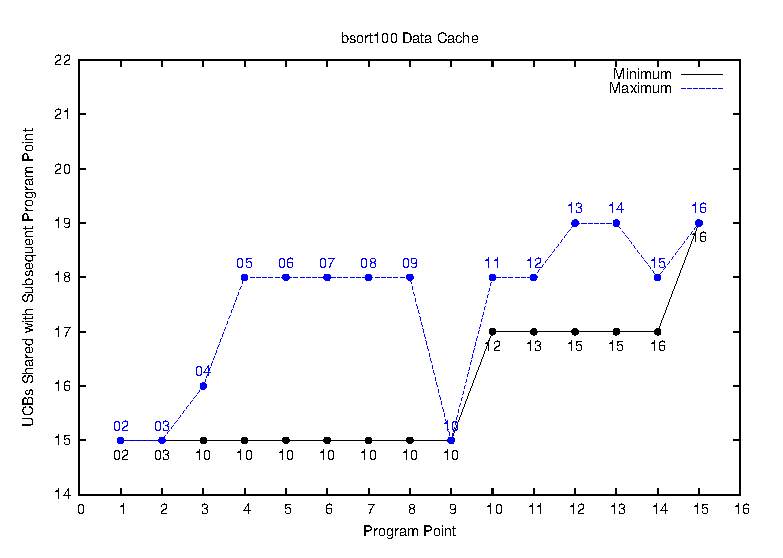
\includegraphics[width=\linewidth]{eps/bsort-dcache.eps}
\end{center}

\begin{center}
  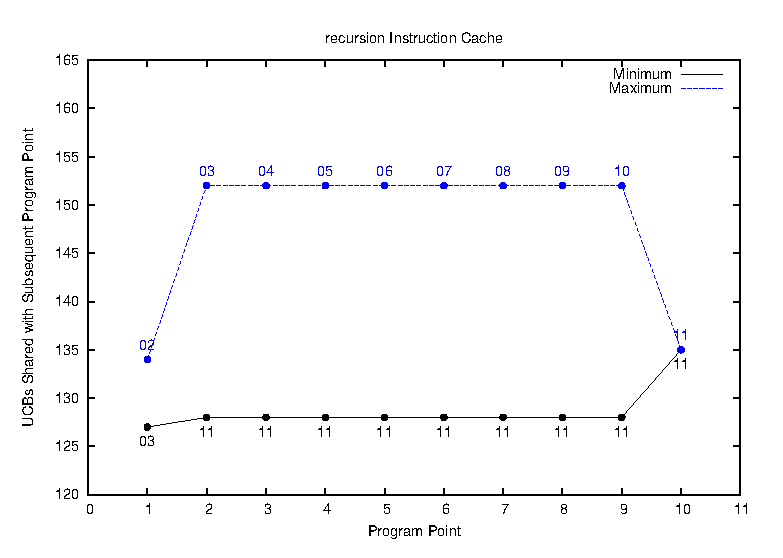
\includegraphics[width=\linewidth]{eps/recursion-icache.eps}
\end{center}

\begin{center}
  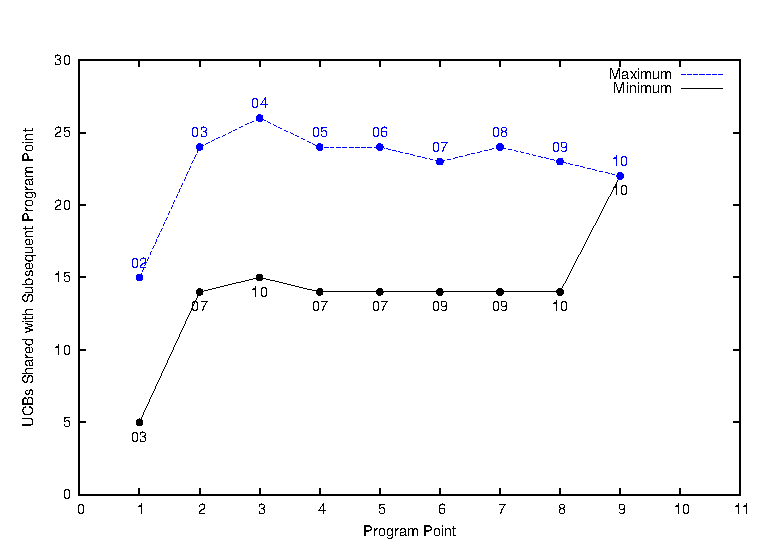
\includegraphics[width=\linewidth]{eps/recursion-dcache.eps}
\end{center}

%% An alternative for a wider graph
%% 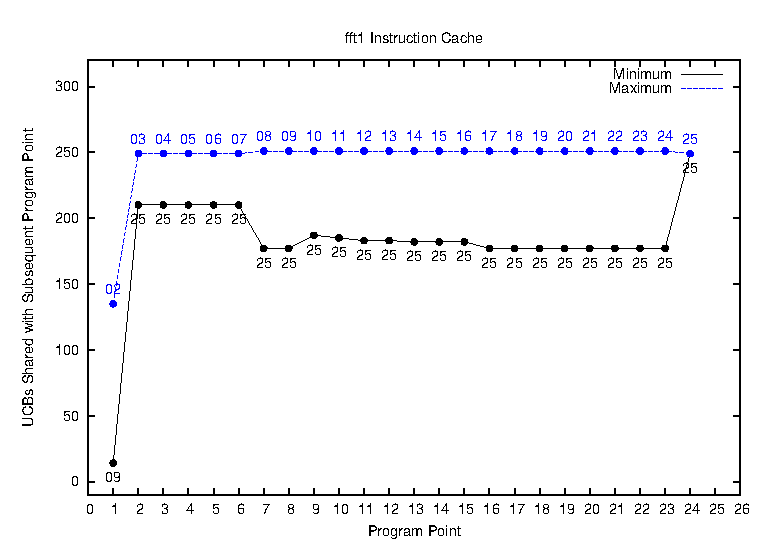
\includegraphics[width=\linewidth]{eps/fft1-icache.eps}

\begin{center}
  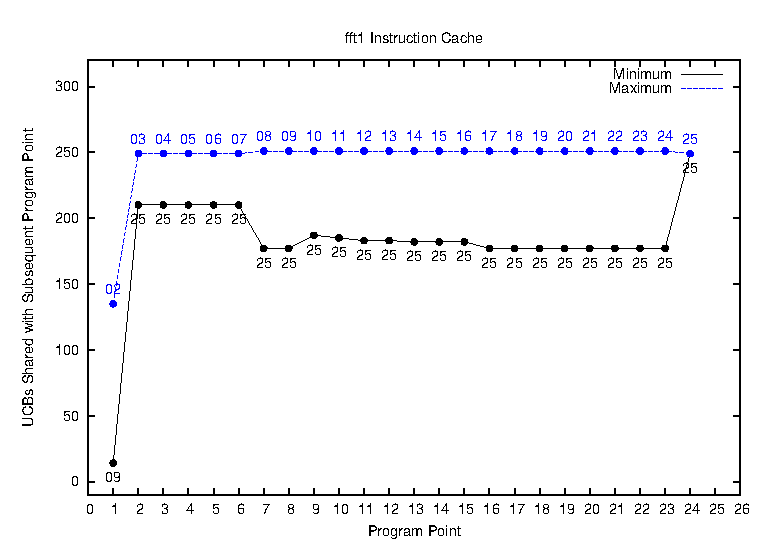
\includegraphics[width=\linewidth]{eps/fft1-icache.eps}
\end{center}

\begin{center}
  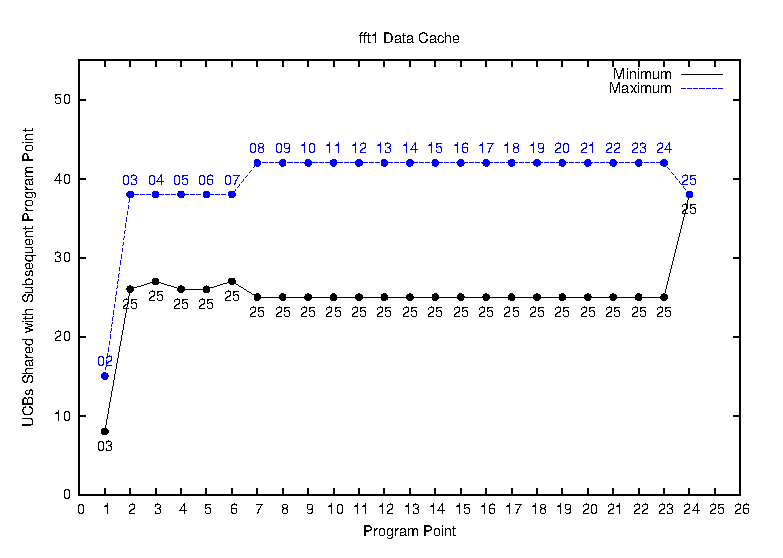
\includegraphics[width=\linewidth]{eps/fft1-dcache.eps}
\end{center}

\begin{minipage}{\linewidth}
\centering
%  \caption {Benefit of Proposed Method}
    \begin{tabular}{l l | l}
      Task & Cache & Benefit \\ \hline
      bsort & ${I}$ & 2 \\ 
      & ${D}$ & 0 \\
      \hline
      fft1  & ${I}$ & 121 \\
      & ${D}$ & 7 \\
      \hline
      recursion & ${I}$ & 7 \\
      & ${D}$ & 10 \\
    \end{tabular}
    \bigskip

    Benefit of Proposed Method
    \bigskip
\end{minipage}

Examining the graphs for all tasks and caches (instruction and data)
there are a few common traits. The minimum shared UCBs sharply
increases at the end of the tasks execution. This is due to the nature
of the over-estimation of shared UCBs and the tasks, the number of
instructions in the basic block between the final program points is
relatively small; limiting the number of cache lines that could be
filtered by the intersection.

Drastic spikes downwards in the shared UCB counts for the minimum and
maximum approaches coincide with function call boundaries, or large
conditional blocks. At these boundaries, the maximum and minimum
approaches have similar UCB counts. This may be an area for further
study, using a greater number of tasks.

There is a sharp upward spike in the early program points for the
maximum approach. This is likely due to the early initialization
blocks built into tasks. The minimum approach shows a clear benefit of
selecting a preemption point outside of the early initialization
section. 

\subsection{Breakdown Utilization}

To determine the schedulability benefit of the explicit preemption
placement approach another case study was performed. This study
focuses on the breakdown utilization when comparing the UCB only
approach for EDF \cite{lunniss:13} to the proposed method of explicit
preemption point placement. For convenience the UCB Only approach for
EDF will be referred to as ${UOE}$, and Explicit Preemption point
Placement as ${EPP}$.

The appropriate schedulablity test for ${UOE}$ is found in
Luniss \emph{et~al.} \cite{lunniss:13}. It is comprised of three
parts: ${\gamma^{ucb}_{t,j}}$, ${U^*_j}$, and ${U^*}$. They represent
the maximum CRPD for a task ${j}$, the utilization of the task ${j}$
including the CRPD of the task, and the utilization of the task set.
A task set is schedulable when ${U^* \le 1}$.

\begin{equation}
  \gamma^{ucb}_{t,j} = BRT \cdot \max\limits_{\forall k \in aff(t,j)}
  \left\{ \left| UCB_k \right| \right\}
\end{equation}

\begin{equation}
  U^*_j = \frac{C_j \cdot \gamma^{ucb}_{t,j}}{T_j}
\end{equation}

\begin{equation}
  U^* = \sum_j U^*_j
\end{equation}

The task set from which the breakdown utilization benefit is
calculated comes, again, from the MRTC suite \cite{mrtc:01}. Borrowing
the technique from \cite{lunniss:13}, each task has its deadline (and
therefor period) set to ${T_i = u \cdot (C_i + \gamma^{ucb}_{t,j})}$
where ${u}$ is a constant. The constant, ${u}$, begins at the number
of tasks (10) and is increased in steps of .25 until the task set
becomes schedulable. Incremental negative adjustments are then made to
determine when the set becomes unschedulable, indicating the breakdown
utilization.

For ${UOE}$, the UCBs for each task are needed (${UCB_k}$.) The
earlier evaluation section \emph{Preemption Cost Characterization}
describes a method for obtaining the UCB counts between two program
points. The UCB count used by ${UOE}$ is the maximum UCB count at any
program point in the task. Using the maximum shared UCB count between
two points is appropriate.

Similarly, for ${EPP}$, the UCBs between each program point are
required. The method described in \emph{Preemption Cost
Characterization} delivers this information, and is used
appropriately.

The last input variables required for both approaches are ${C_i}$ and
${BRT}$. Both of these were obtained through simulation. ${C_i}$ was
captured as the total number of cycles required to complete a task
without preemptions. ${BRT}$ was determined by performing a single
cached instruction and recording the number of cycles used to complete
it, followed by performing the instruction when it was not cached. The
difference yielded a ${BRT}$ of ${<some>}$ cycles.

To hasten the calculation of the breakdown utilization using the
${EPP}$ approach the results of the ${UOE}$ breakdown utilization are
used to seed the determination of ${Q}$. \emph{This section to be
  completed based upon 'The initial CRPD calculation from UOE'...}


\subsection {Taskset Schedulability Evaluation}\label{sec:taskset schedulability}
The schedulability performance metrics we intend to compare various
preemption models with are: 1) the percentage of schedulable task sets
as a function of the task set utilization, 2) the percentage of
schedulable task sets as a function of the number of tasks, 3) the
percentage of schedulable task sets as a function of the maximum CRPD,
and 4) the percentage of schedulable task sets as a function of the
variability of the CRPD variance \begin{math}\sigma_{CRPD}\end{math}.
The following preemption models will be studied namely: 1) fully
non-preemptive, 2) fully preemptive, 3) limited preemption naive
approach, 4) limited preemption point placement with fixed CRPD
preemption cost, 5) limited preemption point placement with variable
CRPD preemption cost, and 6) optimal preemption point placement with
enhanced CRPD preemption cost. 

Our approach for generating the synthetic task sets involves a number
of steps which is summarized as follows.  The number of basic blocks
generated each task is in the
interval \begin{math}[N_{i}(min),N_{i}(max)]\end{math} using a random
uniform distribution.  Each basic block non-preemptive WCET is
generated using a Gaussian distribution with
mean \begin{math}\mu_{WCET}\end{math} and
variance \begin{math}\sigma_{WCET}\end{math}.  The  utilization of
each task has been generated using the approach proposed in [TBD12].
The task periods \begin{math}T_{i}\end{math} were then computed
dividing the non-preemptive WCET \begin{math}C_{i}^{NP}\end{math} by
the utilization \begin{math}U_{i}\end{math} of each task.  Preemption
costs were randomly generated using the following function (TBD), to
achieve a realistic distribution similar to the one derived
empirically).  The enhanced CRPD is generated to be a percentage of
the WCET in the interval [0, 0.50] with a random uniform
distribution. Cache related preemption delay (CRPD) values are
generated for each pair of potential preemption points.  The variable
CRPD preemption cost model uses the CRPD cost from the each preemption
point to the end of the task. The fixed CRPD preemption cost model
uses the maximum CRPD cost of all variable CRPD preemption cost
values.  
